% Choose one to switch between slides and handout
\documentclass[]{beamer}
%\documentclass[handout]{beamer}

% Video Meta Data
\title{Smart Contracts and Decentralized Finance}
\subtitle{Inheritance, Interfaces, and Libraries}
\author{Prof. Dr. Fabian Schär}
\institute{University of Basel}

% Config File
% Packages
\usepackage[utf8]{inputenc}
\usepackage{hyperref}
\usepackage{gitinfo2}
\usepackage{tikz}
 \usetikzlibrary{calc}
\usepackage{amsmath}
\usepackage{mathtools}
\usepackage{bibentry}
\usepackage{xcolor}
\usepackage{colortbl} % Add colour to LaTeX tables
\usepackage{caption}
\usepackage[export]{adjustbox}
\usepackage{pgfplots} \pgfplotsset{compat = 1.17}
\usepackage{makecell}
\usepackage{fancybox}
\usepackage{ragged2e}
\usepackage{fontawesome}
\usepackage{seqsplit}
\usepackage{tabularx}
\usepackage{tcolorbox}
\usepackage{booktabs} % use instead  \hline in tables

% Color Options
\definecolor{highlight}{rgb}{0.65,0.84,0.82}
\definecolor{focus}{rgb}{0.72, 0, 0}
\definecolor{lightred}{rgb}{0.8,0.5,0.5}
\definecolor{midgray}{RGB}{190,195,200}

 %UniBas Main Colors
\definecolor{mint}{RGB}{165,215,210}
\definecolor{anthracite}{RGB}{45,55,60}
\definecolor{red}{RGB}{210,5,55}

 %UniBas Color Palette (for graphics)
\definecolor{strongmint}{RGB}{30,165,165}
\definecolor{darkmint}{RGB}{0,110,110}
\definecolor{softanthracite}{RGB}{140,145,150}
\definecolor{brightanthracite}{RGB}{190,195,200}
\definecolor{softred}{RGB}{235,130,155}

%Custom Colors
\definecolor{lightergray}{RGB}{230, 230, 230}



% Beamer Template Options
\beamertemplatenavigationsymbolsempty
\setbeamertemplate{footline}[frame number]
\setbeamercolor{structure}{fg=black}
\setbeamercolor{footline}{fg=black}
\setbeamercolor{title}{fg=black}
\setbeamercolor{frametitle}{fg=black}
\setbeamercolor{item}{fg=black}
\setbeamercolor{}{fg=black}
\setbeamercolor{bibliography item}{fg=black}
\setbeamercolor*{bibliography entry title}{fg=black}
\setbeamercolor{alerted text}{fg=focus}
\setbeamertemplate{items}[square]
\setbeamertemplate{enumerate items}[default]
\captionsetup[figure]{labelfont={color=black},font={color=black}}
\captionsetup[table]{labelfont={color=black},font={color=black}}

\setbeamertemplate{bibliography item}{\insertbiblabel}

%tcolor boxes
\newtcolorbox{samplecode}[2][]{
  colback=mint, colframe=darkmint, coltitle=white,
  fontupper = \ttfamily\scriptsize, fonttitle= \bfseries\scriptsize,
  boxrule = 0mm, arc = 0mm,
  boxsep = 1.3mm, left = 0mm, right = 0mm, top = 0.5mm, bottom = 0mm, middle=0mm,
  #1,title=#2}
  
\newtcolorbox{keytakeaway}[2][]{
  colback=softred, colframe=red, coltitle=white,
  fontupper = \scriptsize, fonttitle= \bfseries\scriptsize,
  boxrule = 0mm, arc = 0mm,
  boxsep = 1.3mm, left = 0mm, right = 0mm, top = 0.5mm, bottom = 0mm, middle=0mm,
  #1,title=#2}

\newtcolorbox{exercise}[2][]{
  colback=brightanthracite, colframe=anthracite, coltitle=white,
  fontupper = \scriptsize, fonttitle= \bfseries\scriptsize,
  boxrule = 0mm, arc = 0mm,
  boxsep = 1.3mm, left = 0mm, right = 0mm, top = 0.5mm, bottom = 0mm, middle=0mm,
  #1,title=#2}



% Link Icon Command 
\newcommand{\link}{%
    \tikz[x=1.2ex, y=1.2ex, baseline=-0.05ex]{%
        \begin{scope}[x=1ex, y=1ex]
            \clip (-0.1,-0.1)
                --++ (-0, 1.2)
                --++ (0.6, 0)
                --++ (0, -0.6)
                --++ (0.6, 0)
                --++ (0, -1);
            \path[draw,
                line width = 0.5,
                rounded corners=0.5]
                (0,0) rectangle (1,1);
        \end{scope}
        \path[draw, line width = 0.5] (0.5, 0.5)
            -- (1, 1);
        \path[draw, line width = 0.5] (0.6, 1)
            -- (1, 1) -- (1, 0.6);
        }
    }

% Other commands
\newcommand\tab[1][0.5cm]{\hspace*{#1}} % for code boxes


% Read Git Data from Github Actions Workflow
% Defaults to gitinfo2 for local builds
\IfFileExists{gitInfo.txt}
	{\input{gitInfo.txt}}
	{
		\newcommand{\gitRelease}{(Local Release)}
		\newcommand{\gitSHA}{\gitHash}
		\newcommand{\gitDate}{\gitAuthorIsoDate}
	}

% Custom Titlepage
\defbeamertemplate*{title page}{customized}[1][]
{
  \vspace{-0cm}\hfill\includegraphics[width=2.5cm]{../config/logo_cif}
  \includegraphics[width=1.9cm]{../config/seal_wwz}
  \\ \vspace{2em}
  \usebeamerfont{title}\textbf{\inserttitle}\par
  \usebeamerfont{title}\usebeamercolor[fg]{title}\insertsubtitle\par  \vspace{1.5em}
  \small\usebeamerfont{author}\insertauthor\par
  \usebeamerfont{author}\insertinstitute\par \vspace{2em}
  \usebeamercolor[fg]{titlegraphic}\inserttitlegraphic
    \tiny \noindent \texttt{Release Ver.: \gitRelease}\\ 
    \texttt{Version Hash: \gitSHA}\\
    \texttt{Version Date: \gitDate}\\ \vspace{1em}
    
    
    \iffalse
  \link \href{https://github.com/cifunibas/Bitcoin-Blockchain-Cryptoassets/blob/main/slides/intro.pdf}
  {Get most recent version}\\
  \link \href{https://github.com/cifunibas/Bitcoin-Blockchain-Cryptoassets/blob/main/slides/intro.pdf}
  {Watch video lecture}\\ 
  
  \fi
  
  \vspace{1em}
  License: \texttt{Creative Commons Attribution-NonCommercial-ShareAlike 4.0 International}\\\vspace{2em}
  \includegraphics[width = 1.2cm]{../config/license}
}


% tikzlibraries
\usetikzlibrary{decorations.pathreplacing}
\usetikzlibrary{decorations.markings}
\usetikzlibrary{positioning}
\usetikzlibrary{calc}
\captionsetup{font=footnotesize}

%%%%%%%%%%%%%%%%%%%%%%%%%%%%%%%%%%%%%%%%%%%%%%
%%%%%%%%%%%%%%%%%%%%%%%%%%%%%%%%%%%%%%%%%%%%%%
\begin{document}

\thispagestyle{empty}
\begin{frame}[noframenumbering]
	\titlepage
\end{frame}

%%%
\begin{frame}{Introduction}

Solidity offers various constructs to modularize code and reduce dependency between these modules during development.\\

\vspace{1em}

Understanding the basic concepts is essential for analyzing most of the smart contract code deployed on Mainnet.\\

\vspace{1em}

\uncover<2->{
This video outlines:
\begin{itemize}
	\item	\textbf{Import} for making code modules available across files.
	\item	\textbf{Inheritance} as a way combining multiple contracts to one.
	\item	\textbf{Interface contracts} to create standardized interfaces.
	\item	\textbf{Library contracts} to reuse code across multiple contracts.
\end{itemize}
}

\end{frame}
%%%

%%%
\begin{frame}{Importing files}

\vspace{0.5em}
Keep modules (base contracts, interfaces etc.) in separate files and use \genkey{import} at the top of the applying contract file to:

\begin{itemize}
	\item reflect changes across all applying contracts in development.
	\item keep the applying contract file concise and easily readable.
\end{itemize}

\vspace{0.3em}

\uncover<2->{
\begin{samplecode}{Import Statement Example}
	\begin{lstlisting}[language=Solidity]
// Global import of complete file content.
import "./contractA.sol";

// Importing and renaming a specific element. 
import B as newNameB from "./contractA.sol"; 
\end{lstlisting}
\end{samplecode}

$\Rightarrow$ Importing a file or element thereof is the same as copying the code into the applying contract.\\

\vspace{0.5em}

\link \href{https://docs.soliditylang.org/en/v0.8.15/layout-of-source-files.html}{Solidity Documentation on Importing Source Files}.
}

\end{frame}
%%	

%%%
\begin{frame}{Import paths}

\vspace{0.5em}
The import statement requires a path specification for the source file, for which two ways are common:
\vspace{0.5em}

\begin{enumerate}
	\item	\textbf{Current directory:} \genkey{import} \color{red} \texttt{{"./fileName.sol"}} \color{black} to perform a global import of the code in a file from the same directory.
	\item	\textbf{External paths:} Compilers in common IDEs often let you import files from HTTP, IPFS or NPM.
\end{enumerate}

\vspace{0.5em}

\uncover<2->{
\begin{samplecode}{Example: Import OpenZeppelin ERC-20 Interface Contract in Remix IDE}
	\input{../assets/solidity_code/import_from_GitHub.tex}
\end{samplecode}

\vspace{0.5em}
Note that \genkey{import} requires harmonized pragma versions to compile.
}

\end{frame}
%%%	


%%%
\begin{frame}{Contract Inheritance}

\begin{minipage}{0.45\textwidth}
	\begin{figure}[t]
		\centering
		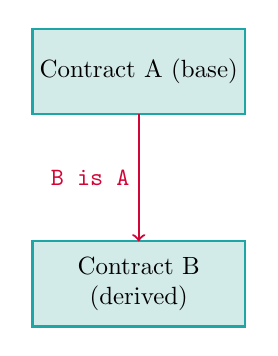
\begin{tikzpicture}[scale=0.9, every node/.style={scale=0.9}]
			% Contract Boxes
	
	\draw[fill = mint!50, thick, draw=strongmint] (0,3) rectangle ++(3,1.2) node [midway, text width = 2.9cm, align = center] {Contract A (base)};
	
	\draw[fill = mint!50, thick, draw=strongmint] (0,0) rectangle ++(3,1.2) node [midway, text width = 2.9cm, align = center] {Contract B (derived)};

% Inheritance arrows
	
	\draw [->][red, thick] (1.5,3) -- (1.5,1.2) node [midway, left] {\texttt{B is A}};



		\end{tikzpicture}
	\end{figure}
\end{minipage}
\begin{minipage}{0.5\textwidth}
	Solidity allows the combination of multiple contracts into a single one via \textbf{inheritance}.

	\vspace{0.5em}

	Inheriting creates base - derived relationships (also called parent – child), where the derived contract takes over \textbf{all \genkey{public} and \genkey{internal} variables and functions}.	

\end{minipage}

\vspace{1em}

	The derived contract compiles the code from all bases and is deployed as a single contract on-chain, i.e.,  all functions are accessed via \textbf{internal function calls}. 

\vspace{1.5em}

\link \href{https://docs.soliditylang.org/en/latest/contracts.html}{Solidity Documentation on Inheritance}.

\end{frame}
%%%	

%%%
\begin{frame}{Building and Inheritance Structure}

\vspace{0.5em}	
\begin{minipage}{0.48\textwidth}
	\begin{samplecode}{Contract Inheritance}
		\begin{lstlisting}[language=Solidity]

contract A {...}

contract B is A {...}

contract C {...}

contract D is B, C {...}
\end{lstlisting}
	\end{samplecode}
\end{minipage}	
\begin{minipage}{0.48\textwidth}
	\begin{figure}[t]
		\centering
		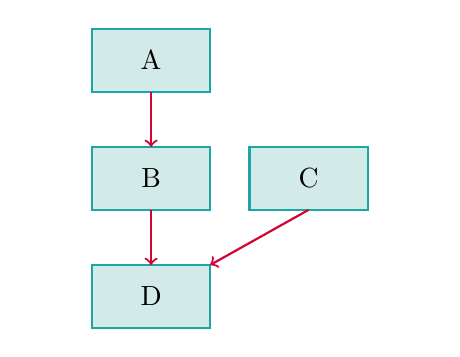
\begin{tikzpicture}[scale=1.0, every node/.style={scale=1.0}]
			% Contract Boxes
	
	\draw[fill = mint!50, thick, draw=strongmint] (0,3) rectangle ++(1.5,0.8) node [midway, text width = 2.9cm, align = center] {A};
	
	\draw[fill = mint!50, thick, draw=strongmint] (0,1.5) rectangle ++(1.5,0.8) node [midway, text width = 2.9cm, align = center] {B};
	
	\draw[fill = mint!50, thick, draw=strongmint] (2,1.5) rectangle ++(1.5,0.8) node [midway, text width = 2.9cm, align = center] {C};
	
	\draw[fill = mint!50, thick, draw=strongmint] (0,0) rectangle ++(1.5,0.8) node [midway, text width = 2.9cm, align = center] {D};

% Inheritance arrows
	
	\draw [->][red, thick] (0.75,3) -- (0.75,2.3);
	
	\draw [->][red, thick] (0.75,1.5) -- (0.75,0.8);
	
	\draw [->][red, thick] (2.75,1.5) -- (1.5,0.8);
	




		\end{tikzpicture}
	\end{figure}
\end{minipage}	

\vspace{2.0em}

\uncover<-2>{
$\Rightarrow$ By inheriting B, D is also based on A.\\

\vspace{0.5em}
$\Rightarrow$ Multiple inheritance is allowed, e.g., D inherits from B and C.\\
}

\end{frame}
%%%


%%%
\begin{frame}{Inheritance Considerations: Overriding}

Both \textbf{modifiers} and \textbf{functions} can be redefined in a derived contract. For this overriding, keep in mind:
\vspace{0.5em}
\begin{itemize}
	\item<2-> Modifiers must have the same name, functions the same signature.
	\item<3-> Explicitly declare functions or modifiers as \genkey{virtual} (in base) and \genkey{override} (in derived).
	\item<4->  Overridden functions can still be accessed via \texttt{super.f()} or \texttt{baseName.f()}.	
\end{itemize}

\vspace{1.5em}

\uncover<5->{
Note that declaring a \textbf{state variable} that visibly exists already in a base (variable shadowing) or \textbf{double use of a name for different members} (function, modifier, or event) within the inheritance structure will not compile.
}

\end{frame}
%%%


%%%
\begin{frame}{Inheritance Considerations: Constructor}

For a derived contract to be deployed\footnote{Missing arguments render it abstract, i.e., containing functions without implementation. Abstract contracts cannot be deployed on their own.}, it must provide the arguments of its base constracts constructors.

\vspace{-0.5em}

\begin{samplecode}{Two Options for Providing Arguments to Base Constructors}
	\begin{lstlisting}[language=Solidity]
contract A {
	uint public a;
	constructor(uint _a){
		a = _a;
	}
}
// Option 1: Include arguments in inheritance list.
contract B is A(3) {
}
// Option 2: Pass arguments as part of constructor.
contract C is A{
	constructor(uint _b) A(_b * 2) {}
}
\end{lstlisting}
\end{samplecode}


\end{frame}
%%


%%%
\begin{frame}{Applying Inheritance to the Auction Contract}

\begin{minipage}{0.3\textwidth}
	\begin{figure}
		\center
		\includegraphics[width= 2.2cm]{../assets/images/construction.png}	
	\end{figure}
\end{minipage}
\begin{minipage}{0.65\textwidth}
	\textbf{Goal:} Modify the sealed bid auction contract, so it can be used as base to be inherited by auction implementations.\\
\end{minipage}

\vspace{3em}

\uncover<2->{
Points to be covered in the derived contract:
\begin{itemize}
	\item	Hardcoded beneficiary address.
	\item	Setting the auction title.
	\item	Option to introduce an auction house fee deducted at the end of the auction.
\end{itemize}
}

\end{frame}
%%%


%%%
\begin{frame}{Placeholder - Coding Auction Base \& Inheritance}

\end{frame}
%%%


%%%
\begin{frame}{Interface Contracts}

\begin{minipage}{0.3\textwidth}
	\begin{figure}
		\center
		\includegraphics[width= 2.2cm]{../assets/images/interface.png}	
	\end{figure}
\end{minipage}
\begin{minipage}{0.65\textwidth}
	\vspace{1em}
	An \textbf{interface} contract is a collection of \genkey{external} functions including their arguments and (optional) return values \textbf{without implementing them}.
\end{minipage}

\vspace{2em}

\uncover<2->{
Basically limited to what a contract ABI can represent, interfaces are \textbf{unable }to:
\vspace{0.5em}
\begin{itemize}
	\item	inherit from other contracts, only other interfaces.
	\item	declare state variables or modifiers.
	\item	declare a constructor.
\end{itemize}


\vspace{1.5em}

\link \href{https://docs.soliditylang.org/en/latest/contracts.html}{Solidity Documentation on Interfaces}.
}

\end{frame}
%%%


%%%
\begin{frame}{Rationale for Interfaces}

\textbf{1. Soundness check via inheritance}\\
\vspace{0.5em}
Inheriting an interface, a contract will not compile unless all interface functions are implemented.\\
\vspace{0.5em}
Note that an ERC-20 compliant contract means nothing else but that the IERC-20 interface is implemented.\\

\uncover<2->{
\vspace{1.5em}
\textbf{2. Encoding pattern for use of external contracts.}\\
\vspace{0.5em}
Imported interfaces provide a contract with the necessary encoding patterns for external calls to contracts implementing this interface. It is a lightweight, reduced dependency alternative to providing the complete code of the target contract.\\
\vspace{0.5em}
Note that an interface can also specify only a subset of the external functions the target contracts have implemented.
}

\end{frame}
%%%


%%%
\begin{frame}{Building a Bidding Contract}

\begin{minipage}{0.3\textwidth}
	\begin{figure}
		\center
		\includegraphics[width= 2.2cm]{../assets/images/bidder.png}	
	\end{figure}
\end{minipage}
\begin{minipage}{0.65\textwidth}
	\vspace{0.5em}
	\textbf{Goal:} Build a personal bidding contract that can be used to participate in an sealed bid auction, using an interface for the auction contract.\\
\end{minipage}

\vspace{2em}

Points to be covered:
\vspace{0.5em}
\begin{enumerate}
	\item	The required interface for the auction contract.
	\item	A bidding contract, that handles
	\vspace{0.5em}
	\begin{itemize}
		\item sealed bid requests and places them with a specified auction.
		\item reveal requests and performs reveals with the specified auction.
		\item reimbursement requests, returning the funds to the caller.
	\end{itemize}
\end{enumerate}


\end{frame}
%%


%%%
\begin{frame}{MyBidder: Auction Contract Interface}

Contract Code subject to review by Matnad

\end{frame}
%%%


%%%
\begin{frame}{MyBidder: Importing Interface and Owner}

Contract Code subject to review by Matnad

\end{frame}
%%%

%%%
\begin{frame}{MyBidder: Bidding and Revealing}

Contract Code subject to review by Matnad

\end{frame}
%%%

%%%
\begin{frame}{MyBidder: Retrieving Funds}

Contract Code subject to review by Matnad

\end{frame}
%%%

%%
\begin{frame}{Library Contracts}

\begin{minipage}{0.25\textwidth}
	\begin{figure}
		\center
		\includegraphics[width= 2.2cm]{../assets/images/library.png}	
	\end{figure}
\end{minipage}
\begin{minipage}{0.7\textwidth}
	\vspace{1em}
	A \genkey{library} is a \textbf{stateless} contract that is a collection of functions and types that are deployed once at a specific address for their code being \textbf{reused by different contracts} using \genkey{delegatecall}. They are \textbf{unable} to:

	\begin{itemize}
		\item	Declare state variables.
		\item	Inherit or be inherited.
		\item	Receive Ether.
	\end{itemize}
\end{minipage}

\vspace{1em}

\uncover<2->{
Consequently:
\begin{itemize}
	\item	Library code is executed in the context of the calling contract.
	\item	Storage variables need to be explicitly supplied.
	\item	Only view and virtual library functions can be called directly.
\end{itemize}

\vspace{1em}

\link \href{https://docs.soliditylang.org/en/latest/contracts.html}{Solidity documentation on libraries}.
}

\end{frame}
%%%


%%%
\begin{frame}{Rationale and Use of Libraries}

Libraries are a tool to reduce gas code by deploying common code across multiple contracts once, such as:
\vspace{0.5em}
\begin{itemize}
	\item	Specific operations based on inputs and outputs (i.e., \genkey{view} and \genkey{virtual} functions).
	\item	Implementation of data types (\typesunits{structs}, \typesunits{enums}, user defined).
	\item	Constants.
\end{itemize}
\vspace{1em}

\uncover<2->{
\textbf{Library Use}\\
\vspace{0.5em}
Applying contract can call libraries analogue to base contracts, i.e., \texttt{libraryName.f()}.\\

\vspace{0.5em}
Attaching library functions to a type within the contract with the directive \texttt{libraryName for} \typesunits{type}. Called on an object of that type, the functions will receive the object as first parameter.
}


\end{frame}
%%%


%%%
\begin{frame}{Wrap Up}
	
While powerful, modularization and reuse of code comes with its own set of complexities.

\vspace{0.5em}
\uncover<2->{
This lecture only touches some key aspects of the topic. For application in your own projects, consult detailed documentations and the numerous examples out there.
}

\vspace{0.5em}
\uncover<3->{
The various open source projects that maintain public repositories with a broad range of mainnet tested smart contract modules may prove a invaluable resource.
}

\uncover<4->{
\begin{exercise}{Exercise 1: Do Not Reinvent the Wheel}
	Spend some time on the website, documentation and GitHub repository of the\\ \link \href{https://www.openzeppelin.com/}{OpenZeppelin} project.\\
	\vspace{0.5em}
	Possible questions to explore:
	\begin{enumerate}
		\item What are the pros and cons for using such libraries?
		\item May any of these contract modules proof useful for a project you are planning?
	\end{enumerate}
\end{exercise}
}

\end{frame}

%%%


%%%
\begin{frame}%[allowframebreaks]
\frametitle{References and Recommended Reading}

 
\link \href{https://docs.soliditylang.org/en/latest/index.html}{Latest Solidity Documentation}.

\vspace{1em}

\link \href{https://github.com/OpenZeppelin/openzeppelin-contracts}{OpenZeppelin GitHub Repository}

\end{frame}
%%%



\end{document}